%************************************************
\chapter[Similarités perçues et objets: application à l’analyse automatique]{Similarités perçues et objets: application à l’analyse automatique}\label{ch:ml_xp}
%************************************************


\section{Introduction}
\label{sec:ch8_intro}

\gl{TODO: bag-frame et early integration} \\ 

\gl{TODO: or Une perception basée sur l'objet} \\ 

\gl{TODO: cependant performances des systèmes de détection faibles} \\

\section{Une représentation basée sur l'objet}

\subsection{Formation des objets}

\subsection{Similarité entres objets}

\subsection{Coefficients de Scattering}

\gl{TODO: scattering+scattering-joint+approche objet}
\gl{TODO: représentation sparse}

\section{Proposition d'un algorithme basé sur une approche objet}

As discussed in Section \ref{sec:ch8_intro}, results in sound perception suggest the appropriateness of an object-based representation of auditory scenes for predicting high-level properties. As the detection of events is still an open problem \cite{7100934},  we consider in this paper a simple quantization scheme that is as generic as possible, implemented using a clustering approach where coherent regions of the scene are identified. The clustering is done using the centroid-based $k$-means clustering algorithm.

Given a set of $d$-dimensional feature vectors $x_l^u\in X_u$, $l=\lbrace 1,2,\ldots,L\rbrace$, extracted from the scene $s_u$, $u=\lbrace 1,2,\ldots,U\rbrace$, the goal of $k$-means is to partition $X_u$ into $M$ clusters $c^u_m\in C_u$, $m=\lbrace 1,2,\ldots,M\rbrace$. The partitioning is done by minimizing for each cluster the squared error between its empirical mean (centroid) and the contained points. Given $\mu_m^u$ the centroid of the cluster $c_m^u$, $k$-means attempts to minimize the following objective function:
\begin{equation}
J(C_u)=\sum\limits_{m} \sum_{x^u_l\in c^u_m} \Vert x_l^u - \mu_m^u \Vert^2\mbox{.}
\end{equation}
Each scene $s_u$ is then described by a set of clusters $C_u$. One should note that this quantization approach differs from unsupervised learning schemes such as the ones studied in \cite{bisot2016acoustic}, where the scene features are projected in a dictionary learned from the entire dataset.

Here, with the aim of better balancing the influence of salient sound events and texture-like sounds on the final decision, the similarity between two scenes is computed based on the similarity of their centroids.

The similarity between all the scene centroids $\mu_i$, $i=\lbrace1,2,\ldots,I \rbrace$ with $I=UM$, is computed using a radial basis function (RBF) kernel $K$ combined with the local scaling method proposed in \cite{selfTuneManor2004}:
\begin{equation}
\label{eq:kc}
K_{ij} = \exp\left( - \dfrac{\Vert \mu_i - \mu_j \Vert^2}{\Vert \mu_i - \mu_{k,i} \Vert \Vert \mu_j - \mu_{k,j} \Vert} \right) 
\end{equation} 
where $\mu_{k,i}$ and $\mu_{k,j}$ are the $k^{\textrm{th}}$ nearest neighbor to the centroids $\mu_i$ and $\mu_j$, respectively, and $\Vert \cdot \Vert$ denotes the Euclidean norm.

To compute the similarity between two scenes, we then consider several centroid-based similarity metrics:
\begin{itemize}
\item \emph{ob-closest} (ob-c): the similarity between two scenes is equal to the largest similarity between their centroids,
\item \emph{ob-averaged} (ob-a): the similarity between two scenes is equal to the average of their centroid similarities, and
\item \emph{ob-weighted} (ob-w): for each scene, each centroid is weighted according to the number of frames belonging to its cluster. Each scene $s_u$ is thus described by a signature $p_u$ of $M$ clusters ($p_u=\lbrace(\mu_1^u,w_1^u),(\mu_2^u,w_2^u),\ldots,(\mu_M^u,w_M^u)\rbrace$), with $\mu_m^u$ and $w_m^u$ being the centroid and the weight of the $m$th cluster respectively. The similarity between scenes is then given by a cross-bin histogram distance, taking into account both the cluster weights and the distances between their centroids.
\end{itemize}

For \emph{ob-w}, the cross-bin histogram distance used is a variant of the earth mover's distance ($\EMD$), known as $\widehat{\EMD}$ and introduced in \cite{pele2008linear}. The $\EMD$ computes the distance between two histograms by finding the minimal cost to be paid to transform one histogram into the other. An advantage of $\EMD$ is that it automatically aligns the histogram bins by using a ``ground distance'' which is the distance between the bin centers in the two histograms. In our case, the histograms are the clusters weights $w^u$ defined over the bins formed by clusters centroids $\mu^u$.

The $\widehat{\EMD}$ variant of $\EMD$ is adapted for non-normalized histograms. To compute the $\widehat{\EMD}$, we use the implementation proposed in \cite{pele2009fast}. Given two signatures $p_u$ and $p_v$ made of $n$ and $m$ clusters respectively, the $\widehat{\EMD}$ is computed by solving the following linear program:
\begin{equation}
\begin{split}
\widehat{\EMD}(p_u,p_v) &=\left( \min\limits_{\lbrace f_{nm}\rbrace} \sum\limits_{n,m} f_{nm}D_{nm}^{uv} \right) \\
&+ \left|\sum\limits_{n} w_n^u - \sum\limits_{m} w_m^v  \right| \alpha \max\limits_{n,m}\lbrace  D_{nm}^{uv}\rbrace.
\end{split}
\end{equation}

\begin{equation*}
\mathrm{s.t.} \quad f_{nm}\geq0 \quad \sum\limits_{m} f_{nm} \leq w_n^u \quad \sum\limits_{n} f_{nm} \leq w_m^v
\end{equation*}

\begin{equation*}
\sum\limits_{n,m}f_{nm} = \min\left( \sum\limits_{n} w_n^u ,\sum\limits_{m} w_m^v \right)
\end{equation*} 

where $\lbrace f_{nm} \rbrace$ is the flow between the cluster weights $w_n^u$ and $w_m^v$, that is, the amount transported from the $n^{\textrm{th}}$ bin to ``supply the demand'' of the $m^\textrm{th}$ bin. We denote by $D^{uv}$ the ground distance, a matrix containing the pairwise distances between the centroids sets $\mu^u$ and $\mu^v$. $D^{uv}$ is computed from the kernel $K$:
\begin{equation*}
D^{uv}=\boldsymbol{1}-K^{(uv)}
\end{equation*}
with $K^{(uv)}$ being the slice of $K$ containing the pairwise similarities between the centroids sets $\mu^u$ and $\mu^v$ of the scenes $s_u$ and $s_v$, respectively. As suggested in \cite{pele2009fast}, we set the tradeoff parameter $\alpha$ to $1$.

To get the final similarity measure between the scenes $s_u$ and $s_v$, an extended Gaussian kernel $K^s$ \cite{chapelle1999support,jing2003support} is computed:
\begin{equation}
\label{eq:ks}
K_{uv}^s = \exp\left( - \dfrac{\widehat{\EMD}(p_u,p_v)}{A} \right) \\
\end{equation}
with $A$ a scaling parameter, set to the mean value of the $\widehat{\EMD}$ between all the scenes. The resulting kernel $K^s$ is known as an $\EMD$ kernel, and it should be noted that there is no guarantee that this kernel is positive definite.

\section{Expérience}

\subsection{objectif}

\gl{TODO: parler de Intégration \emph{early} \vs \emph{late}}

The \emph{ob} approaches are compared to commonly used early integration approach (\emph{early}).

\gl{TODO: ici expliquer pourquoi on ne parle pas de classification}

\subsection{Banques de données}

The experiments in this paper are carried out on the private part of the DCASE 2013 dataset\cite{giannoulis2013database, 7100934} and the public part of the DCASE 2016 dataset \cite{Mesaros2016_EUSIPCO}.

The DCASE 2013 dataset consists of two parts, namely a public and a private subset, each made up of $100$ $30$-second recordings of various acoustic scenes. The $100$ recordings are evenly divided into $10$ acoustic scene classes. To build the DCASE 2013 dataset, three different recordists visited a wide variety of locations in Greater London over a period of several months and in each scene recorded a few minutes of audio. No
systematic variations in the recordings covaried with scene
type: all recordings were made under moderate weather conditions, at varying times of day and week, and each recordist recorded each scene type. As a consequence, DCASE2013 dataset enjoys an interesting intra-class diversity while remaining manageable in terms of size, making it suitable for extensive evaluation of algorithmic design choices \cite{lagrange:hal-01082501}. 

In addition, it is still a challenging dataset, with a state-of-the-art system based on feature design and SVMs achieving $76\%$ \cite{roma2013} (winner of the DCASE2013 challenge), while recent approaches based on label tree embedding achieve between $84\%$ and $87\%$ on DCASE 2013 depending on the prior knowledge used during training \cite{phan2016label}.

The dataset is split into a public dataset that can used for optimizing the ASC system and a private dataset used for computing the resulting accuracy using a five-fold cross validation scheme. The folds used in this paper are the same as the ones used during the challenge.


\subsection{Descripteurs}

Experiments are carried out using scattering coefficients as well as mel-frequency cepstral coefficients (MFCCs) as features. For the scattering transform, each $30$-second scene is described by $128$ vectors computed with half-overlapping windows $\boldsymbol{\phi}(t)$ of duration $T=372\,\mathrm{ms}$, for a total of $24\,\mathrm{s}$. Indeed, $3$ seconds are discarded at the beginning and end of the scene to avoid boundary artifacts. Experiments are conducted with and without logarithmic compression (see Section \ref{sec:logcomp}).

MFCCs are computed for windows of $50\,\mathrm{ms}$ and hops of $25\,\mathrm{ms}$, with full frequency range. Different ranks of coefficients were tested to compute the MFCCs, results here are only reported for the best setting, which consisted of $40$ MFCCs, including the first coefficient related to the average energy. This setting gives us $600$ feature vectors per scene. To get a more robust representation, a pooling step is performed on the MFCCs: each recording is divided into $250$-second long non-overlapping ``texture'' windows \cite{1021072}, over which the feature vectors are averaged. This yields number of vectors comparable to that of the scattering transform.


\subsection{Systèmes, paramètres et métriques}

The influence of the temporal scattering transform and the \emph{ob} approaches are assessed in an unsupervised setting (ASSR).

For the \emph{ob} approaches, we use the precomputed kernels described in Section \ref{sec:object}. For both the \emph{early} and \emph{late} approaches, a linear kernel as well as an RBF kernel are used. 

Clustering is done using $k$-means$++$ \cite{arthur2007k}, an augmented version of $k$-means with a more robust initialization procedure. Three numbers of clusters are tested: $8$, $16$ and $32$.

\subsection{Métriques}

For ASSR, evaluation is performed on the private part of the DCASE 2013 dataset. The metric used is the precision at rank $k$ ($p@k$), which is computed by taking a query item and counting the number of items of the same class within the $k$ closest neighbors, and then averaging over all query items. The $p@k$ is computed for $k=\lbrace 1,\ldots,9\rbrace$, since each class only has $10$ items. Note that a $p@1$ is equivalent to the classification accuracy obtained by the classifier which chooeses the label of the closest neighbor for a given item. For each experimental setting, we only report the results obtained with the sets of parameters, \emph{i.e.} the number of clusters $M$ for the \emph{ob} approaches and the scaling parameter $k$ of the RBF kernels (see Eq. \ref{eq:kc}) leading to the best $p@9$.

\subsection{Résultats}

\begin{figure}[t]
\begin{center}
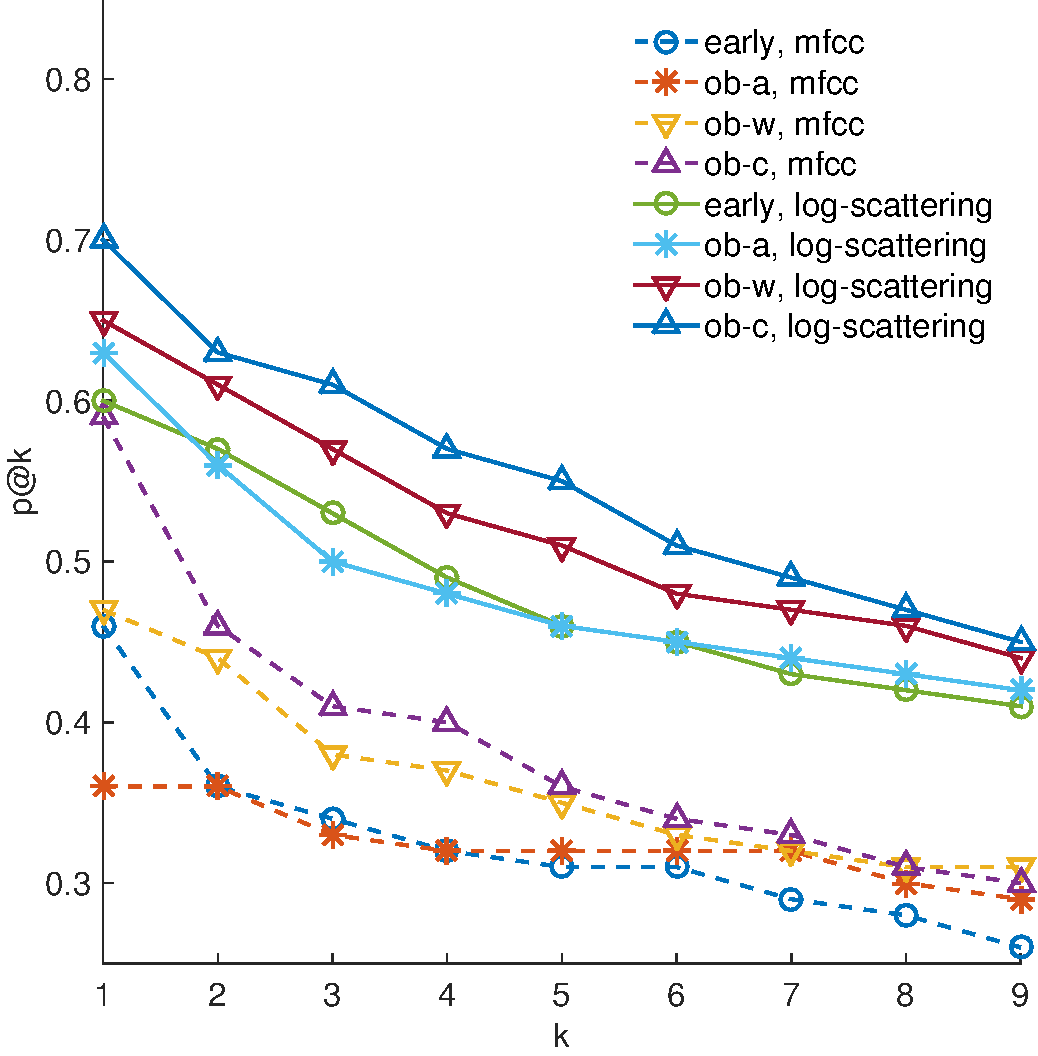
\includegraphics[width=.9\columnwidth]{gfx/ch_8/unsupervised_test2-eps-converted-to}
\caption{Acoustic scene similarity retrieval (ASSR) in the DCASE 2013 private dataset: precisions at rank $k$ ($p@k$) obtained for MFCCs and scattering with logarithmic compression, as a function of the rank $k$.}
\label{fig:ASS_1}
\end{center}
\end{figure}

%\begin{figure}[t]
\begin{center}
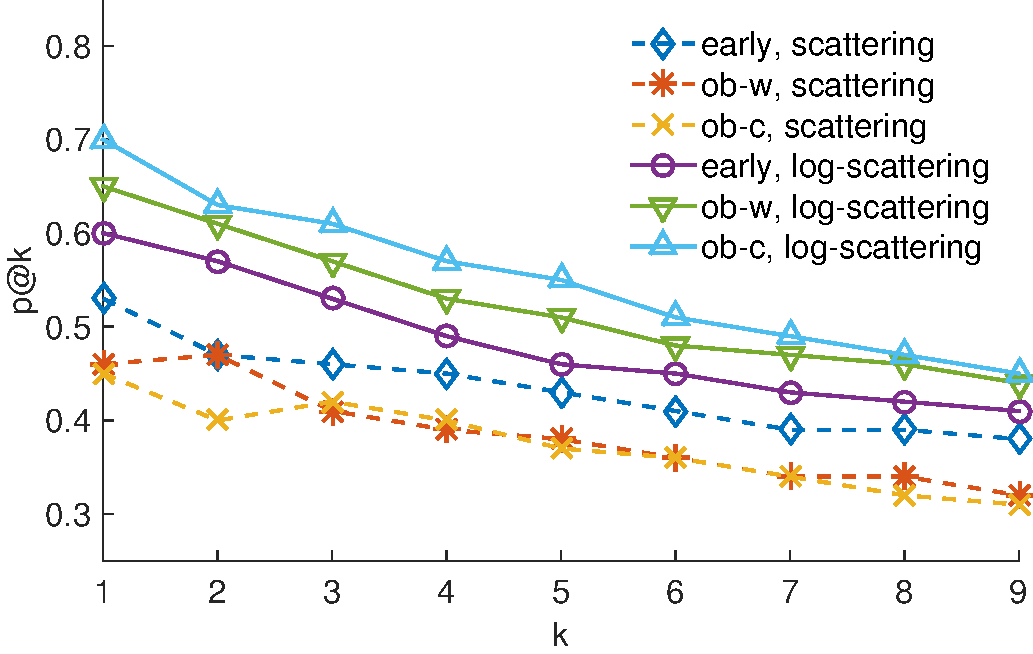
\includegraphics[width=.9\columnwidth]{gfx/ch_8/unsupervised_test1-eps-converted-to}
\caption{Acoustic scene similarity retrieval (ASSR) in the DCASE 2013 private dataset: precisions at rank $k$ ($p@k$) obtained for scattering coefficients, with and without logarithmic compression, as a function of the rank $k$.}
\label{fig:ASS_2}
\end{center}
\end{figure}

This section presents evaluation results for the ASSR settings. The $p@k$ for different settings are shown in Figures \ref{fig:ASS_1} and \ref{fig:ASS_2}, illustrating the effect of the different similarity metrics and the influence of the logarithm, respectively.

\subsubsection{MFCC \vs scattering transform}

Irrespective of the rank $k$ considered, best result is achieved for the scattering transform with logarithmic compression using the \emph{ob-c} approach. Overall, log-compressed scattering coefficients systematically outperform MFCCs. This is to be expected since the scattering coefficients capture larger-scale modulations, as opposed to MFCCs which only describe the short-time spectral envelope.

\subsubsection{Role of logarithmic compression}

Outcomes for the scattering with and without logarithmic compression are shown in Figure \ref{fig:ASS_2}. It can be seen that the logarithmic compression strongly improves the results, especially for the \emph{ob} approaches, which perform worse than \emph{early} without the logarithmic compression.

\subsubsection{Object-based \vs early integration}

For the scattering transform, both \emph{ob-c} and \emph{ob-w} outperform \emph{early}, thus confirming the benefits of using an object-based representation to refine the similarity measures between the scenes. However, it is worth noticing that \emph{ob-a} performs comparably to \emph{early}, showing that the discriminant information is destroyed by averaging the contributions from all centroids. To take advantage of an object-based representation, we need to select certain representative centroids when comparing objects. Furthermore, it appears that \emph{ob-c} is better able to characterize the classes than \emph{ob-w}. This last observation suggests that weighting a centroid according to the number of frames it contains may prove to be a limited solution. Indeed, nothing a priori indicates that the discriminant information between two scenes lays within the majority of their frames. On the contrary, two similar environments may shared a lot of similar sound sources with only a few sources discriminating between them.

The same observations are made for the MFCCs for $k\leq5$. However for a rank $k$ greater than $5$, all the \emph{ob} approaches perform equivalently. This may be due to the fact that, at some point, the MFCCs fail to dissociate the discriminative events of a scene from the non-informative ones, thus making the cluster selection/weighting step useless.






\subsection{Application à la classification}

%*****************************************
%*****************************************
%*****************************************
%*****************************************
%*****************************************




